\documentclass{beamer}
\usetheme{Warsaw}

\usepackage{xcolor}
\usepackage{listings}
\usepackage{textcomp}
\usepackage{ulem}
\usepackage{listings}

\title{Lowering high-level language constructs to LLVM IR}
\author{Ramkumar Ramachandra}
\titlegraphic{
\includegraphics[scale=0.20]{llvm-logo}}

\lstset{
    inputencoding=utf8,
%    backgroundcolor=\color{white},
    tabsize=4,
    rulecolor=,
    numbers=left,
    upquote=true,
%    aboveskip={1.5\baselineskip},
    columns=fixed,
    showstringspaces=false,
    extendedchars=true,
    breaklines=true,
    prebreak = \raisebox{0ex}[0ex][0ex]{\ensuremath{\hookleftarrow}},
    frame=single,
    showtabs=false,
    showspaces=false,
    showstringspaces=false,
    basicstyle=\scriptsize\ttfamily,
    identifierstyle=\ttfamily,
    keywordstyle=[1]\ttfamily\color{blue},
    keywordstyle=[2]\ttfamily\color{purple},
    keywordstyle=[3]\ttfamily\colorbox{yellow},
    commentstyle=\ttfamily\color[rgb]{0.133,0.545,0.133},
    stringstyle=\ttfamily\color[rgb]{0.627,0.126,0.941},
}

\lstdefinelanguage{rhine}{
  morestring=[b]",
  morekeywords=[1]{defn, fn, let, first, rest, cons, if},
  morekeywords=[2]{true, false},
  morekeywords=[3]{map, map2},
}

\lstdefinelanguage{ocaml}{
  morestring=[b]",
  morekeywords=[1]{let, in, fun},
  morekeywords=[3]{const_8, magic_lim, llenv},
}

\makeatletter
\lstdefinelanguage{llvm}{
  morecomment = [l]{;},
  morestring=[b]", 
  sensitive = true,
  morekeywords=[1]{
    define, declare, global, constant,
    internal, external, private,
    linkonce, linkonce_odr, weak, weak_odr, appending,
    common, extern_weak,
    thread_local, dllimport, dllexport,
    hidden, protected, default,
    except, deplibs,
    volatile, fastcc, coldcc, cc, ccc,
    x86_stdcallcc, x86_fastcallcc,
    ptx_kernel, ptx_device,
    signext, zeroext, inreg, sret, nounwind, noreturn,
    nocapture, byval, nest, readnone, readonly, noalias, uwtable,
    inlinehint, noinline, alwaysinline, optsize, ssp, sspreq,
    noredzone, noimplicitfloat, naked, alignstack,
    module, asm, align, tail, to,
    addrspace, section, alias, sideeffect, c, gc,
    target, datalayout, triple,
    blockaddress
  },
  morekeywords=[2]{
    add, fadd, sub, fsub, mul, fmul,
    sdiv, udiv, fdiv, srem, urem, frem,
    and, or, xor,
    icmp, fcmp,
    eq, ne, ugt, uge, ult, ule, sgt, sge, slt, sle,
    oeq, ogt, oge, olt, ole, one, ord, ueq, ugt, uge,
    ult, ule, une, uno,
    nuw, nsw, exact, inbounds,
    phi, call, select, shl, lshr, ashr, va_arg,
    trunc, zext, sext,
    fptrunc, fpext, fptoui, fptosi, uitofp, sitofp,
    ptrtoint, inttoptr, bitcast,
    ret, br, indirectbr, switch, invoke, unwind, unreachable,
    malloc, alloca, free, load, store, getelementptr,
    extractelement, insertelement, shufflevector,
    extractvalue, insertvalue,
  },
  morekeywords=[3]{@malloc},
  alsoletter={\%},
  keywordsprefix={\%},
}
\makeatother

\begin{document}

\begin{frame}
  \titlepage
\end{frame}

\begin{frame}{it's pretty readable}
  \lstinputlisting[language=llvm]{scary.ll}
  \lstinputlisting[language=llvm]{scary2.ll}
\end{frame}

\begin{frame}{the simplest program}
  \lstinputlisting[language=c]{add.c}
  \lstinputlisting[language=llvm]{add.ll}
\end{frame}

\begin{frame}{a few interesting instructions}
  \lstinputlisting[language=c]{add-print.c}
  \lstinputlisting[language=llvm]{add-print.ll}
\end{frame}

\begin{frame}{map!}
  \begin{center}
\includegraphics[scale=0.6]{map}\end{center}
  \vfill
  \lstinputlisting[language=haskell,frame=none,numbers=none]{map.hs}
\end{frame}

\begin{frame}{the functor}
  \begin{columns}
    \begin{column}[b]{5.5cm}
      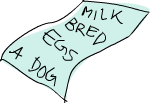
\includegraphics[scale=0.6]{list}
    \end{column}
    \begin{column}[b]{4.5cm}
      \lstinputlisting[language=rhine]{list.rh}
    \end{column}
  \end{columns}
\end{frame}

\begin{frame}{types dance}
  \begin{columns}
    \begin{column}[b]{5.5cm}
      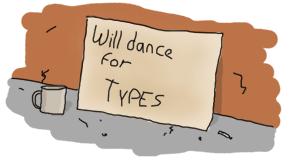
\includegraphics[scale=0.6]{types-dance}
    \end{column}
    \begin{column}[b]{4.5cm}
      \begin{itemize}
      \item[] \texttt{i64}
      \item[] \texttt{double}
      \item[] \texttt{i1}
      \item[] \texttt{i8}
      \item[] \texttt{i8*}
      \end{itemize}
    \end{column}
  \end{columns}
\end{frame}

\begin{frame}{sum type (tagged union?)}
  \begin{columns}
    \begin{column}[b]{5.5cm}
      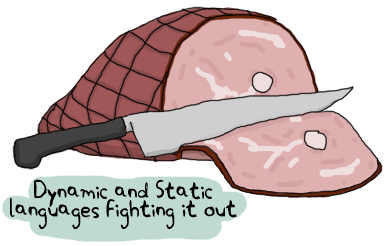
\includegraphics[scale=0.4]{dynamic-static-types}
    \end{column}
    \begin{column}[b]{4.5cm}
      \lstinputlisting[language=llvm]{value_t_intro.ll}
    \end{column}
  \end{columns}
\end{frame}

\begin{frame}{the array type}
  \lstinputlisting[language=llvm]{value_t_array.ll}
\end{frame}

\begin{frame}{a look at the implementation}
  \lstinputlisting[language=rhine]{map.rh}
\end{frame}

\begin{frame}{the function type}
  \lstinputlisting[language=llvm]{value_t_simplefunction.ll}
\end{frame}

\begin{frame}{a vaargs refresher}
  \lstinputlisting[language=c]{vaargs.c}
\end{frame}

\begin{frame}{varargs in llvm}
  \begin{columns}
    \begin{column}[b]{5.5cm}
      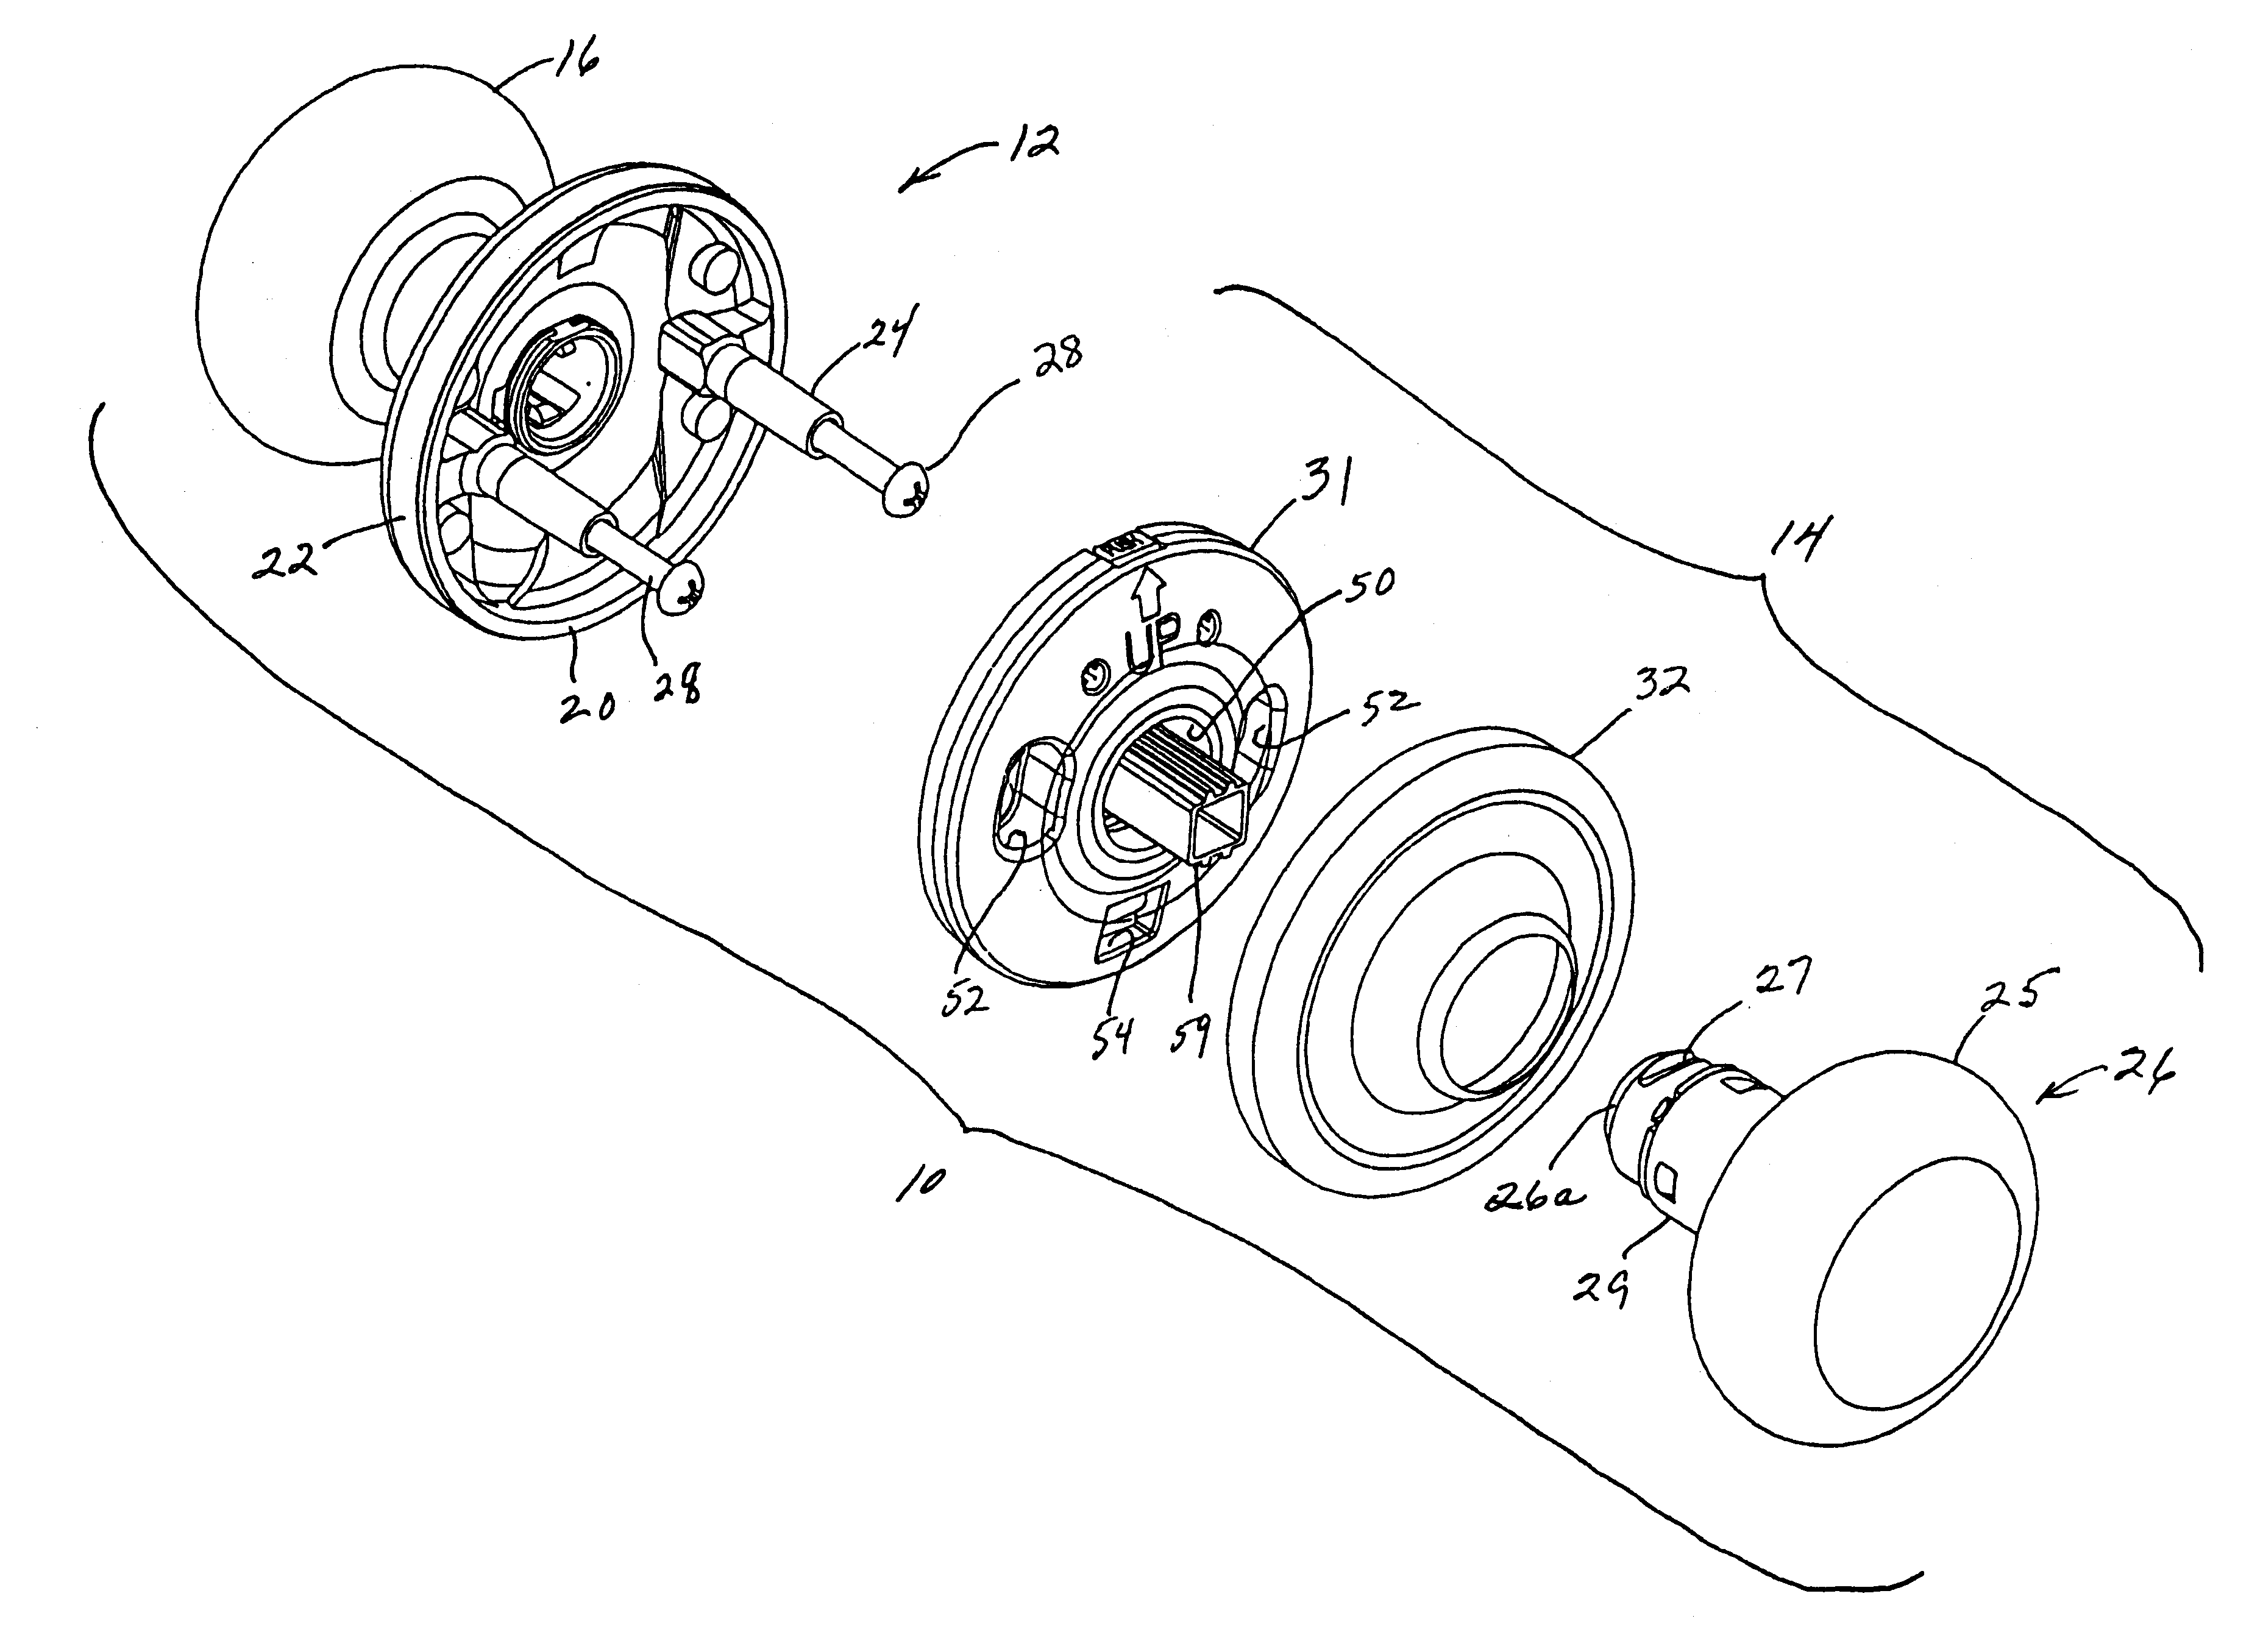
\includegraphics[scale=0.05]{variable-knob}
    \end{column}
    \begin{column}[b]{4.5cm}
      \begin{itemize}
      \item[] \texttt{@llvm.va\_start}
      \item[] \texttt{@llvm.va\_end}
      \item[] \texttt{\sout{@llvm.va\_arg}}
      \end{itemize}
    \end{column}
  \end{columns}
\end{frame}

\begin{frame}{the x86 detail}
  \lstinputlisting[language=llvm,frame=none,numbers=none]{vararg.ll}
  \vfill
  \lstinputlisting[language=ocaml]{vararg.ml}
\end{frame}

\begin{frame}{$\lambda$ lifting}
  \begin{columns}
    \begin{column}[b]{3.8cm}
      
\includegraphics[scale=0.4]{lambda}
    \end{column}
    \begin{column}[b]{6.2cm}
      \lstinputlisting[language=rhine]{lambda.rh}
      \lstinputlisting[language=rhine]{lambda-defn.rh}
    \end{column}
  \end{columns}
\end{frame}

\begin{frame}{closure}
  \begin{columns}
    \begin{column}[b]{3.8cm}
      
\includegraphics[scale=0.3]{closure}
    \end{column}
    \begin{column}[b]{6.2cm}
      \lstinputlisting[language=rhine]{closure-init.rh}
    \end{column}
  \end{columns}
\end{frame}

\begin{frame}{closure implementation}
  \lstinputlisting[language=ocaml]{closure.ml}
\end{frame}

\begin{frame}{the final value\_t}
  \lstinputlisting[language=llvm]{value_t.ll}
\end{frame}

\begin{frame}{end notes}
  \begin{enumerate}
  \item https://github.com/artagnon/rhine
  \item http://llvm.org/docs/LangRef.html
  \item clang -S -emit-llvm
  \item \#llvm on Freenode IRC
  \end{enumerate}
\end{frame}

\end{document}
